\section{Arquitectura del sistema}
\subsection {Arquitectura física}
Las herramientas del proyecto OMI pueden ser dispuestas sobre diferente arquitectura física. Por un lado se puede hacer uso 
del intérprete como una herramienta de un sistema operativo GNU/Linux, siguiendo así una arquitectura de escritorio. 
Por otro se puede usar el sistema en como una arquitectura cliente/servidor.

\subsubsection{Escritorio}
El cliente OMI puede ser utilizado en una arquitectura de escritorio, funcionando como un comando del sistema. Para ello solo se precisa de un PC con un sistema operativo GNU/Linux.

\subsubsection{Cliente/servidor}
El intérprete OMI puede ser usado en una arquitectura cliente/servidor, en la que hace de servidor. El servidor OMI espera una petición para un proceso de interpretación. Esta petición
contendrá el código fuente que se desea interpretar.

El servidor OMI procesa un código fuente para su interpretación devolviendo una estructura de datos en formato JSON que representa el árbol de nodos resultado del análisis léxico y sintáctico. 
Luego espera peticiones para resolver cada paso dentro del proceso de interpretación y devolver una estructura de datos en el mismo formato que representa qué ha ocurrido mediante el estado actual.

El sistema servidor es independiente del cliente en el sentido de que pueden usarse distintos clientes para el mismo servicio. El proyecto OMI presenta un cliente web llamado runTree 
que funciona en cualquier navegador moderno, no obstante se puede usar otra tecnología como cliente. 

Para ejecutar el sistema en una arquitectura cliente servidor se precisa de un equipo que tenga conexión a internet con un navegador web que hará de cliente. Por otro lado se necesita de un equipo servidor
que presente una alta disponibilidad. Este equipo dispondrá de uns sitema GNU/Linux sobre el que se ejecutará el intérprete y un servidor web Apache que servirá de plataforma para dar el servicio web.

\subsection {Arquitectura lógica}
En esta sección se presenta la arquitectura del sistema. Se presentan 
dos niveles de organización la parte frontal (front-end) y la parte 
interna o motor (back-end). 

La parte frontal se encarga de analizar y procesar la entrada del usuario.
Una vez tratada la entrada, se pasa la ejecución a las estructuras que conforman 
el motor del sistema. Estas llevarán a cabo una serie de tareas que puden producir
un resultado que será enviado al frontal. La parte frontal mostrará 
los datos como salida del programa en un formato establecido.

\begin{center}
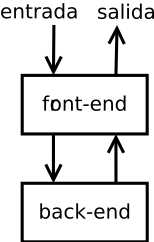
\includegraphics[scale=0.7]{dia/generic.png} \\
\end{center}

Aunque bien se podría haber especificado otra capa correspondiente a la gestión de datos
llevada a cabo por las tablas de símbolos, esta se ha incluido en la parte del motor. Los datos que 
las tablas de símbolos tratan no mantienen persistencia, están muy ligados al proceso interno de 
interpretación y no representan los datos correspondientes al modelo de datos, sino que sirve para
referenciar componentes de la capa del motor de la aplicación.

\subsubsection{Frontal (front-end)}
El frontal del sistema se compone de un analizador léxico y un analizador sintáctico. 
Aunque es posible especificar reglas léxicas mediante reglas gramaticales, se ha separado el 
estos dos componentes por los siguientes motivos:

\begin{itemize}
\item La reglas lexicográficas suelen ser muy simples y para su descripción no se precisa de una 
notación tan compleja como las gramaticales.
\item Las expresiones regulares son más concisas y fáciles de entender que las gramáticas
\item A partir de expresiones regulares se puede describir analizadores léxicos eficientes.
\item Se modulariza el proceso en dos componentes con objetivos bien definidos. 
\end{itemize}

Además del analizador léxico y sintáctico el front-end contiene estructuras funcionales correspondientes
a la toma de datos de entradas y a la impresión de la salida. 

\paragraph {Analizador léxico}
El analizador léxico implementa una gramática de tipo 3 en la jerarquía de Chomsky, estas
se corresponden con las gramáticas regulares. 

Las gramáticas regulares, también llamadas gramáticas finitas, se pueden describir mediante expresiones regulares. 
Cada expresión regular denota un lenguaje $L(r)$. Una expresión regular se construye a partir de otras expresiones
más simples, utilizando un conjunto definidos de reglas. Estas reglas indican la manera de conseguir el conjunto 
$L(r)$ combinando de varias formas los lenguajes denotados por las subexpresiones de $r$. Las expresiones regulares
se pueden definir de una forma recursiva como sigue: 

\begin {enumerate}
\item $\epsilon$ es una expresión regular que denota el lenguaje que unicamente contiene la cadena vacía.
\item Si $a$ fuese un símbolo del alfabeto, entonces $a$ es una expresión regular que denota el lenguaje formado
por la cadena $a$.
\item Si $r$ y $s$ son dos expresiones regulares que denotan los lenguajes $L(r)$ y $L(s)$ respectivamente entonces:
\begin{itemize}
   \item $L(r|s)\ \rightarrow\ L(r)\ \cup\ L(s)$
   \item $L(rs) \ \rightarrow\ L(r)L(s)$
   \item $L(r*)\ \rightarrow\ (L(r))*$
   \item $L(r+)\ \rightarrow\ (L(r))+$
   \item $L(r?)\ \rightarrow\ \{\epsilon\}\ \cup\ L(r)$
   \item $L((r))\ \rightarrow\ (L(r))$
\end{itemize}
\end{enumerate}

Las gramáticas regulares pueden ser implementadas mediante un autómata finito. Un autómata finito se define formalmente como sigue:
$$AF = (S,\Sigma,\delta,S_0,F)$$

De forma que:
\begin{itemize}
\item $S$ es un conjunto de estados.
\item $\Sigma$ es el conjunto de símbolos que conforman el alfabeto.
\item $\delta$ es una función de transición tal que $(\delta\ :\ S\times\Sigma \rightarrow S)$. Donde para cada estado y según 
cada carácter de entrada del alfabeto le hace corresponder un nuevo estado.
\item $S_0$ es el estado inicial.
\item $F$ es un conjunto de estado finales.
\end{itemize}

El analizador léxico se corresponde con un autómata finito donde, al alcanzarse un estado final, se produce la generación de un token.
Un token es un elemento léxico con cierto valor para el lenguaje. Normalmente se corresponde con una cadena de
caracteres que se puede corresponder con una palabra reservada, un identificador, un número... Un token puede contener un 
valor. Los token son utilizados por el analizador sintáctico para llevar a cabo el procesamiento del código fuente. 

Las reglas lexicográficas a partir de las cuales se construye el analizador léxico son descritas junto la gramática, haciendo uso
de expresiones regulares y diagramas sintácticos.

\paragraph{Analizador sintáctico}
El analizador sintáctico implementa una gramática de tipo 2 en la jerarquía de Chomsky, esta se corresponden con las 
gramáticas independientes del contexto. Una gramática de este tipo, como su propio nombre indica, no depende del contexto para
su resolución, lo que origina que los recursos que permiten analizarlas sean relativamente eficientes y simples. Una gramática de
este tipo pueden ser analizadas mediante algoritmos con un orden $O(n^3)$ donde $n$ es el tamaño de la entrada. No obstante existen 
un subconjuntos de este tipo de gramáticas como las $LL(k)$ y $LR(k)$ que pueden ser analizados en tiempo $O(n)$. Estos últimos son los
comúnmente utilizados en los lenguajes de programación.

En el análisis sintáctico se pueden utilizar métodos descendentes o ascendentes, en función de cómo se genera el árbol sintáctico. 

Los métodos de análisis descendentes tienen como objetivo construir el árbol de derivación desde la raíz hacia las hojas. Normalmente se
utilizan analizadores del tipo $LL$ dado que la entrada es tratada desde la izquierda y las reglas de producción también desde la izquierda.
Estos tipos de analizadores tienen el problema de la incertidumbre, debido a que dado un símbolo no terminal debe determinar qué regla de derivación aplicar. 
La incertidumbre puede ser reducida mediante métodos como el retroceso o la predicción.
 
Los métodos de análisis de ascendentes pretenden construir el árbol de derivación o de sintáxis desde las hojas hacia la raíz. Para este tipo normalmente se utiliza 
analizadores del tipo $LR$ dado que la entrada es tratada desde la izquierda, mientras que las reglas de producción son tratadas desde la derecha. Este tipo de
analizadores reducen la incertidumbre dado que se parte de una una regla de derivación para obtener el símbolo no terminal que se corresponde a la misma. 

Para el lenguaje tratado en este proyecto se tomará un analizador sintáctico ascendente $LR$, dado que es uno de los más utilizados, son eficientes y 
existen herramientas que permiten su generación automática a partir de la descripción de la gramática. 

Las gramáticas libres de contexto son analizadas mediante un autómata de pila. La configuración en un momento dado del analizador se corresponde con el contendido de la pila y el resto de la 
entrada que aún está por analizar. La entrada estará constituida por tokens obtenidos por el analizador léxicos, teóricamente estos serán almacenados en una estructura de buffer, pero 
en la práctica estos son generados bajo demanda por el analizador léxico. En la pila se irá almacenando una serie de estados en función del procesamiento realizado sobre la cadena de entrada. 
El autómata puede llevar a cabo dos operaciones:

\begin{description}
\item[Desplazar:] Consiste en sacar del buffer de entrada un símbolo terminal e introducir el estado correspondiente en la pila.
\item[Reducir:] Consiste en reducir $n$ estados del tope de la pila al estado correspondiente, según las reglas de producción.
\end{description}

El análisis finaliza cuando se produce un estado de aceptación o de error. 

En la práctica este tipo de analizador sintáctico se implementa mediante un programa monitor que encierra la lógica descrita, un buffer de entrada en el que se almacenan
los tokens, una pila que almacena los estados producidos, y dos tablas. La primera tabla guardará las acciones y determina, para el estado actual y el primer símbolo del buffer, 
la acción a realizar (desplazar o reducir). La otra tabla, la tabla de saltos, es utilizada tras llevarse a cabo una de reducción, y determina a partir del estado en el tope de la pila
tras la reducción y la regla que se utilizó para la misma, el siguiente estado a introducir en la pila. 

\begin{center}
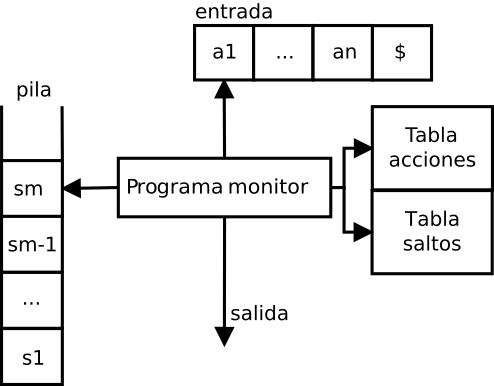
\includegraphics[scale=0.7]{dia/asd.png} \\
\end{center}

Por cada reducción que se lleve a cabo se creará un nodo del árbol sintáctico. De esta forma el árbol es creado desde las hojas hacia la raíz. Cada nodo encierra un significado semántico que 
será llevado a cabo cuando se ejecuten. Estos nodos constituyen a su vez el motor, o back-end, del sistema.

\paragraph{Mecanismos de entrada/salida}
En el nivel de front-end también se dan los diferentes componentes para capturar la entrada del usuario, así como para facilitar la salida que produce en sistema.

La entrada más común supondrá código fuente que será interpretado y ejecutado. Este se podrá dar de varias formas:

\begin{itemize}
\item Mediante la entrada estándar del sistema.
\item Contenido en fichero.
\item Mediante un intérprete de línea.
\end{itemize}

Es posible que se den datos de entrada que no sean código fuente, como por ejemplo, una extensión que debe ser cargada, la opción de mostrar ayuda ...

Por otro lado los datos de salida que produce el programa normalmente serán volcados en la salida estándar sistema en forma de cadenas de caracteres. 
Esta será el resultado visual de la interpretación del código fuente, aunque es posible que un determinado código fuente no produzca salida de este tipo. 

El programa debe ser capaz de procesar los errores y mostrarlos por la salida de errores del sistema. Para ello debe controlar las líneas y ficheros procesados en cada
momento. Los errores pueden ser de diferente tipos:

\begin{itemize}
\item Errores léxicos.
\item Errores sintácticos.
\item Errores semánticos.
\end{itemize}

Además los errores pueden presentar diferente grado:

\begin{description}
\item [Avisos:] Informan de que algún recurso del lenguaje no se utiliza de la forma habitual, y aunque no se produce un error como tal, puede suponer un error de codificación.
\item [Normales:] No finalizan la ejecución del código fuente pero provocan que la sentencia en la que sucede no se pueda ejecutar.
\item [Críticos:] Finalizan la ejecución del código fuente.
\end{description}

\subsubsection{Motor (back-end)}
El motor del sistema lo conforman los nodos creados mediante el análisis sintáctico. Estos nodos se denominan nodos ejecutables, dado que su procesamiento conlleva la realización operacional
de la semántica que encierran. Los nodos ejecutables se categorizan según el tipo de operaciones que conlleva su ejecución, así existen nodos aritméticos, lógicos, de control de flujo, 
de definiciones... 

El sistema presenta una jerarquía de nodos ejecutables que establece la naturaleza de los mismos, dotándolos de características de una forma general y que serán concretadas en los niveles más
bajos de la jerarquía. Se presenta de esta forma, nodos ejecutable genéricos como expresiones, referencias, imprimibles....

El procesamiento de un nodo ejecutable, que fue creado a partir del análisis sintáctico, puede originar la creación de otros nodos ejecutables, a estos 
últimos se les denominará nodos ejecutables dinámicos. Un nodo dinámico es creado y referenciado por una estructura de datos denominada tabla de símbolos. 
Esta estructura también es considerada un componente del motor del sistema.

Los nodos ejecutables presentan dos niveles de procesamiento semántico: la inicialización y la ejecución. Además también se ha de controlar cómo estos son creados y eliminados de 
forma dinámica en la tabla de símbolos. 



\paragraph{Inicialización}
Todo nodo ejecutable se inicializa a partir de otros nodos ejecutable sobre los que operará. Normalmente estos nodos se corresponderán con los hijos del nodo en cuestión en el árbol sintáctico. 

La inicialización de un nodo ejecutable se lleva a cabo durante la creación del árbol sintáctico, por tanto los nodos se inicializan de una forma ascendente, es decir,
antes los nodos hijos que los padre.

Durante la inicialización se lleva a cabo algunas comprobaciones de tipos, asignaciones y otras operaciones. No obstante, todo proceso que se lleve a cabo durante la
inicialización debe ser independiente de la ejecución. Se ha de tener en cuenta que un nodo ejecutable sólo se inicializa una vez, y sin embargo se puede ejecutar varias
veces, siendo esta última dependiente del estado en un momento dado. Se puede decir pues que la inicialización tiene un carácter estático.

\paragraph{Ejecución}
Una vez generado el árbol sintáctico, lo que conlleva la inicialización de los nodos ejecutables que lo componen, se procede a la ejecución del mismo. La ejecución comienza desde el 
nodo raíz hacia las hojas, se hace pues un recorrido del árbol en profundidad.

La ejecución de un nodo es iniciada normalmente desde su nodo padre, y generalmente conlleva la ejecución de sus nodos hijos antes de proceder a su propia ejecución. Así por ejemplo 
la ejecución de un nodo suma conllevará el cálculo del lado izquierdo de la expresión, lo que se corresponde con la ejecución uno de sus nodos hijo, luego se calculará
el lado derecho, correspondiente a la ejecución del otro nodo hijo, para, una vez ejecutados sus hijos (los operandos), proceder al cálculo de la suma, lo que se corresponde 
con su propia ejecución. 

Durante la ejecución de un nodo ejecutable lo normal es que primero se resuelvan los nodos referencias, aquellos que se corresponden con nodos dinámicos de tipos no definidos. Estos 
nodos referencian a otros nodos creados dinámicamente en la interpretación y que se encuentran accesibles desde la tabla de símbolos. Algunos nodos referencias, 
también denominados nodos de expresiones no definidas, son los correspondientes a: variables, funciones u clases de objetos. Una vez se ha obtenido el nodo al que estos referencian, 
se procede con la ejecución como si los nodos obtenidos fueran los hijos del nodo en proceso.

Aunque la ejecución del árbol se hace inicialmente con un recorrido en profundidad existen nodos que rompen esta secuencia, haciendo que la ejecución pase a nodos específicos 
o repitiendo la ejecución de varios de sus hijos. Cabe decir que una vez se salte la secuencia de ejecución el recorrido seguirá siendo en profundidad. Estos nodos 
se corresponden con sentencias de control de flujo, llamadas a funciones, etc.

El resultado de ejecutar un nodo no tiene por que ser estático, dependiendo en gran medida del contexto, es decir, del estado de la tabla de símbolos. Se puede decir pues que la 
ejecución de un nodo tiene un carácter dinámico dependiente de la tabla de símbolos.

\paragraph{Tabla de símbolos}
La tabla de símbolos es una estructura de datos que almacena referencias a nodos creados dinámicamente en el proceso de interpretación. Estos nodos serán creados en la 
ejecución del árbol de sintáctico y serán accedidos desde la ejecución de determinados nodos en la resolución de referencias. 

Las tablas de símbolos se componen de pares donde el primer elemento es un identificador que nomina al símbolo y el segundo elemento es una referencia al nodo ejecutable. 

Aunque en una tabla de símbolos es posible guardar referencias a cualquier nodo se mantiene diferentes tipos tablas de símbolos según la naturaleza de los nodos a los que se
referencian. Esto hace posible que se puedan repetir identificadores para distintos tipos de nodos como variables, funciones o clases.

Dos identificadores que pueden estar en la misma tabla de símbolos o distintas, pueden referenciar al mismo nodo. El propio nodo debe ser capaz de guardar cuantas referencias al 
mismo tiene. Esto se hace por criterios de optimización, para la reutilización de datos y para realizar una eliminación del nodo de una forma segura cuando sea necesario.

Las tablas de símbolos pueden quedar organizadas en niveles, aunque únicamente un nivel, el actual en un momento dado, es el que se utilizará para la resolución de referencias.
Esto hace posible definir diferentes ámbito para el acceso a determinados símbolos. Los niveles quedan dispuestos en una estructura de pila, de forma que el nivel actual es
la cima de la pila. Una vez un nivel es eliminado de la pila se eliminan todas las referencias del mismo y el nivel anterior queda en la cima y por tanto es considerado el nivel actual.

Existen nodos que presentan sus propias tablas de símbolos, esto hace que muchas definiciones sean internas al mismo. Por ejemplo las clases de objetos mantienen sus propias tablas
de símbolos para referencias los métodos y atributos, y los arrays presentan una tabla de símbolos para guardar las claves y sus valores. Es común que en la ejecución 
de uno de estos nodos se sustituya la tabla de símbolos en uso por la del nodo en cuestión.

La tabla de símbolo es una estructura de datos que forma parte del motor de la aplicación dado que gestiona y almacena datos presentes en este nivel. 

\paragraph{Eliminación de referencias}
Los nodos creados de forma dinámica por el proceso de interpretación deben ser eliminados cuando ya no se precisen de ellos. Por ejemplo cuando se produce una asignación destructiva. Como
los nodos creados de forma dinámica son reutilizados y pueden ser referenciados por más de un símbolo se ha de controlar que no exista ninguna referencia al mismo 
antes de proceder a su eliminación. Así cada nodo guarda el número de referencias al mismo.

Los nodos correspondientes al árbol sintáctico nunca serán eliminados durante la ejecución y no será hasta la finalización del programa hasta que se proceda a la liberación de los recursos 
que consumen.





\subsubsection{runTree}
runTree es un sistema que hace de cliente del intérprete OMI, cuando este funciona como servidor. Se encarga de llevar a cabo peticiones para navegar por el proceso de interpretación de un código
fuente dado. 

El cliente runTree presenta una arquitectura interna en dos capas al igual que el intérprete. El backend de este se comunica con el forntend del intérprete cuando funciona de servidor

\begin{center}
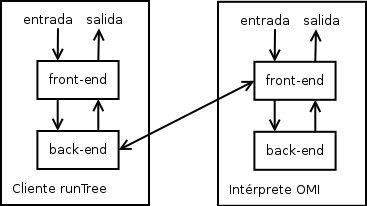
\includegraphics[scale=0.7]{generic_cliente_servidor.png} \\
\end{center}

El frontend del cliente runTree lo componen elementos relacionados con la interfaz del usuario. Captura eventos de esta y lo envía al backend para su procesamiento, a su vez representa los datos que recibe del backend. 

El backend del cliente runTree lo componen elementos que guardan el estado interno del proceso de interpretación. Normalmente estos elementos son inicializados mediante datos que recibe del servidor como fruto de 
una petición.





